%!TeX root=../tese.tex
%(dica para o editor de texto: este arquivo é parte de um documento maior)
% para saber mais: https://tex.stackexchange.com/q/78101/183146

% https://otexts.com/fpp2/index.html
% https://www.tensorflow.org/tutorials/structured_data/time_series

\chapter{Séries temporais}
\label{cap:series}

Neste capítulo são apresentados os conceitos básicos de séries temporais. Também são discutidos brevemente os modelos tradicionais de análise e descrição das séries, ou de previsões de valores futuros, de acordo com o objetivo do estudo. Tais modelos são, por exemplo, baseados em médias móveis, tendências e sazonalidades presentes nos dados.

De acordo com Pedro A. Morettin e Clélia M C. Toloi \citep{morettin}, uma série temporal é qualquer conjunto de observações ordenadas no tempo. São exemplos: valores diários de poluição de uma cidade, valores mensais de temperatura, índices diários da bolsa de valores, número médio anual de manchas solares e registro de marés em portos e estuários.

A análise e predição de cotações de moedas estrangeiras, índices de ações, entre outros dados econômicos, constituem uma área essencial da economia e que exige a avaliação de um número enorme de fatores, muitos dos quais de características humanas e portanto imprevisíveis em sua exatidão, sendo descritos como exemplos de fenômenos \emph{estocásticos}, isto é, probabilísticos.

As séries temporais podem ser \defi{contínuas} em função do tempo, como é o exemplo de registros de marés, ou \defi{discretas} como são todos os outros exemplos, ou seja, os valores são tomados a $N$ intervalos regulares de um período $T$ considerado, tal que $N = T/\Delta t$. Na prática, para o uso em modelos, segundo explica Morettin e Toloi \citep{morettin}, as séries contínuas devem ser discretizadas em intervalos, uma vez que é esse tipo de dado que poderá ser processado num computador.

Pode-se classificar a análise das séries temporais de acordo com seu objetivo de estudo. Morettin e Toloi \citep{morettin} listam os alguns objetivos principais:

\begin{itemize}
	\item{Investigar o mecanismo gerador da série temporal, procurando descrevê-la a partir de uma função teórica.}
	\item{Fazer previsões de valores futuros da série, seja tanto a curto quanto a longo prazo.}
	\item{Descrição da série, em termos de tendências, variações sazonais, ou então análises descritivas por meio de histogramas, médias móveis, etc.}
	\item{Procurar por periodicidades relevantes nos dados, quando não fazemos suposições de periodicidades comuns como semanais, mensais ou anuais, por exemplo.}
\end{itemize}

Neste contexto, Morettin e Toloi \citep{morettin} definem que um modelo é uma descrição probabilística de uma série temporal, cabendo ao cientista de dados decidir a melhor utilização desse modelo segundo seus objetivos. 

Além disso eles afirmam que qualquer tarefa de previsão, sendo este o objetivo, será baseada em algum procedimento computacional que calcula uma estimativa do futuro baseada na otimização de uma função de perda a partir de combinações lineares de valores do passado. É a união de um modelo probabilístico com a otimização de uma função de perda que define um \defi{método de previsão}.

Há dois tipos básicos de modelos que lidam com séries temporais, de acordo com Morettin e Toloi \citep{morettin}, que são os modelos \defi{paramétricos}, onde a análise é feita no \emph{domínio temporal} com suposições e parâmetros a serem estimados, e os modelos \defi{não-paramétricos}, em que a análise é feita no \emph{domínio das frequências} com um enfoque mais descritivo e sem muitas suposições.

Dentre os modelos paramétricos, destacam-se os modelos \emph{ARIMA} (\emph{autorregressivos integrados de médias móveis}), disponíveis como bibliotecas das linguagens \eng{Python} e \eng{R}, enquanto que entre os modelos não-paramétricos destaca-se a \emph{análise espectral}, também denominada de \emph{análise de Fourier}, já que as ferramentas utilizadas são as transformadas de Fourier e suas variações.

Na última seção desse capítulo, uma estrutura de uma rede neural recorrente, implementada com a API Keras, é proposta como um modelo \defi{semiparamétrico}, ou seja, estimando parâmetros inerentes às redes neurais, mas não utilizando parâmetros ou suposições específicas sobre os dados, para a realização de previsões de valores futuros de séries temporais financeiras, com enfoque nas séries históricas de cotações de moedas estrangeiras.\footnote{Tais séries estão disponíveis para \eng{download} no site do Banco Central do Brasil: \url{https://www.bcb.gov.br/}}.

\section{Processos estocásticos}

De acordo com Morettin e Toloi \citep{morettin}, um \defi{processo estocástico} é uma familia $Z = \{ Z(t), t \in \mathcal{T} \}$, onde o conjunto $\mathcal{T}$ é normalmente tomado como $\mathcal{T} = \mathbb{Z}$ ou $\mathcal{T} = \mathbb{R}$, tal que, para cada $t \in \mathcal{T}$, $Z(t)$ é uma variável aleatória (v.a.). 

Portanto, um processo estocástico é uma família de variáveis aleatórias reais $Z(t),\; t \in \mathcal{T}$, definidas num mesmo espaço de probabilidades $(\Omega, \mathcal{A}, \mathcal{P})$, e portanto $Z(t)$ é uma função de dois argumentos, isto é, $Z(t, \omega),\; t \in \mathcal{T},\; \omega \in \Omega$.

Para cada $t \in \mathcal{T}$ fixado, $Z(t, \omega)$ será uma v.a. com uma distribuição de probabilidades. Pode haver uma função de densidade de probabilidade diferente para cada $t \in \mathcal{T}$, mas normalmente assume-se que é a mesma, conforme anotado por Morettin e Toloi \citep{morettin}.

Por outro lado, para cada $\omega_i \in \Omega$ fixado, denotamos $Z(t, \omega_i)$ por $Z^{(i)}(t)$ como uma função de $t$, denominada de \defi{trajetória} do processo, ou simplesmente de \emph{série temporal}. Isto define uma série temporal como uma trajetória ou realização de um processo estocástico, o que pode ser melhor ilustrado pela Figura \ref{fig:trajetorias}, abaixo.

\begin{figure}[htb]
\centering
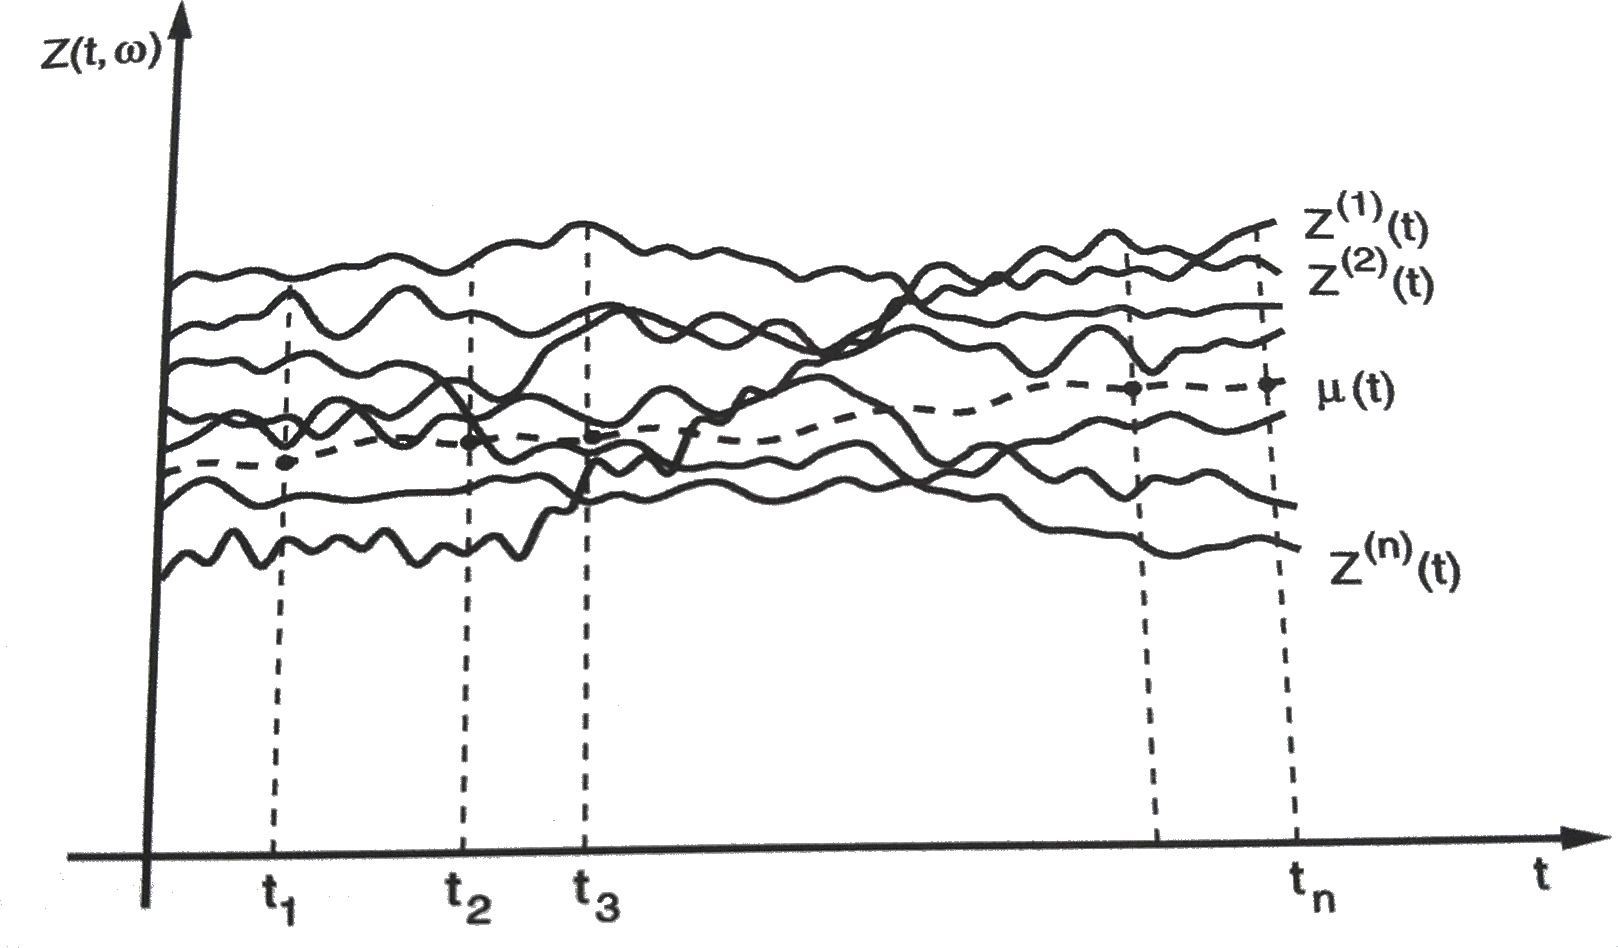
\includegraphics[width=10cm]{figuras/trajetorias}
\caption{Processo estocástico como uma família de trajetórias, isto é, de séries temporais.\footnote{Extraido de Morettin e Castro Toloi, 2019, pág 27.}}
\label{fig:trajetorias}
\end{figure}

Estaremos interessados em processos univariados tanto em $\mathcal{T}$ quanto em $\Omega$, isto é, séries temporais de apenas um argumento temporal, e com um evento $\omega \in \Omega$ fixado e portanto omitido, o que simplifica a notação de $\{Z^{(i)}(t), t \in \mathcal{T}\}$ para $\{Z(t), t \in \mathcal{T}\}$, o que definem as \emph{séries temporais univariadas}, que descrevem como uma v.a. real evolui no domínio temporal $\mathcal{T}$.

Além disso, para as séries e modelos aqui tratados iremos restringir $\mathcal{T} = \mathbb{Z}$, assim omitiremos a definição de um domínio geral e fixaremos a notação como sendo $\{Z(t), t \in \mathbb{Z}\}$ ou ainda $\{Z_t, t \in \mathbb{Z}\}$, para denotar as \emph{séries temporais discretas univariadas}, que além de discretas são equiespaçadas no tempo. A partir de agora, serão chamadas simplesmente de \defi{séries temporais}, pois são os únicos processos estocásticos de interesse neste trabalho.

\subsection{Definições}

Sejam $t_1, \ldots, t_n$ elementos quaisquer de $\mathcal{T}$, então se conhecermos as \emph{distribuições finito-dimensionais} dadas por:

\begin{equation}\label{series:2.1}
F(z_1, \ldots, z_n; t_1, \ldots, t_n) = P\{ Z_{t_1} \leq z_1, \ldots, Z_{t_n} \leq z_n \}
\end{equation}

Teremos então que o processo estocástico $Z = \{ Z_t, t \in \mathcal{T} \}$ estará especificado, para todo $n \geq 1$. Tais funções de distribuição devem, de acordo com Morettin e Toloi \citep{morettin} satisfazer as condições:

	(i) (Simetria) Para qualquer permutação $j_1, \ldots, j_n$ dos índices $1, \dots, n$:
\[ F(z_{j_1}, \ldots, z_{j_n}; t_{j_1}, \ldots, t_{j_n}) = F(z_1, \ldots, z_n; t_1, \ldots, t_n) \]

	(ii) (Compatibilidade) Para $m < n$:
\[ \lim_{\mathlarger{z_{m+1} \to \infty, \ldots, z_n \to \infty}} F(z_1, \ldots, z_m, z_{m+1}, \ldots, z_n; t_1, \ldots, t_n) = F(z_1, \ldots, z_m; t_1, \ldots, t_m) \]

Segundo Morettin e Toloi \citep{morettin}, pode-se demonstrar que qualquer conjunto de funções de distribuição da forma \ref{series:2.1} satisfazendo as duas condições acima define um processo estocástico $Z$ sobre $\mathcal{T}$.

Em termos práticos, não se conhecem as funções de distribuição finito-dimensionais de um processo $Z$ sobre $\mathcal{T}$. Assim a abordagem mais utilizada, conforme Morettin e Toloi \citep{morettin} é tentar determinar os momentos, principalmente os de primeira e segunda ordem, das v.a. $Z_{t_1}, \ldots, Z_{t_n}$. 

O momento de primeira ordem, isto é, a \defi{média} de $Z$ é definida por: 

\begin{equation}\label{series:2.5}
\mu(1; t) = \mu(t) = \E\{Z(t)\} = \int_{-\infty}^{\infty} z f(z;t)dz, t \in \mathcal{T}
\end{equation}

Define-se, a partir dos momentos de primeira ordem, a \defi{função de autocovariância} (facv) de $Z$:

\begin{equation}\label{series:2.6}
\gamma(t_1, t_2) = \mu(1,1; t_1,t_2) - \mu(1; t_1)\mu(1; t_2) = \Cov\{Z(t_1),Z(t_2)\}
\end{equation}

Particularmente, quando $t = t_1 = t_2$, define-se a função \defi{variância} de $Z$, configurando um momento de segunda ordem, por:

\begin{equation}\label{series:2.7}
\gamma(t, t) = \Var\{Z(t)\} = \E\{Z^2(t)\} - \E^2\{Z(t)\}
\end{equation}

\subsection{Processos estacionários}



%\section{Um modelo de série temporal construído com uma rede neural}